
\newcommand{\vdmkw}[1]{\texttt{\textbf{#1}}}
\chapter{Automatic Generation of Code}\label{sec:codegen}

It is possible to generate Java code\index{code generation} for a
large subset of VDM-SL and VDM++ models. In addition to Java, C and
C++ code generators are currently being developed. Both these code
generators are in the early stages of development. The C++ generator
is not included with releases of Overture yet, but the C generator is
far enough along that it can be included for testing purposes. For
comparison, code generation of VDM-SL and VDM++ specifications to both
Java and C++ is a feature that is available in
VDMTools~\cite{Java2VDMMan,CGMan,CGManPP}. The majority of this
chapter focuses solely on the Java code generator available in
Overture, with a brief discussion of the C code generator ending the
chapter.

\section{Use of the Java Code Generator}
\label{sec:javacg_use}

\begin{figure}[htbp]
\begin{center}
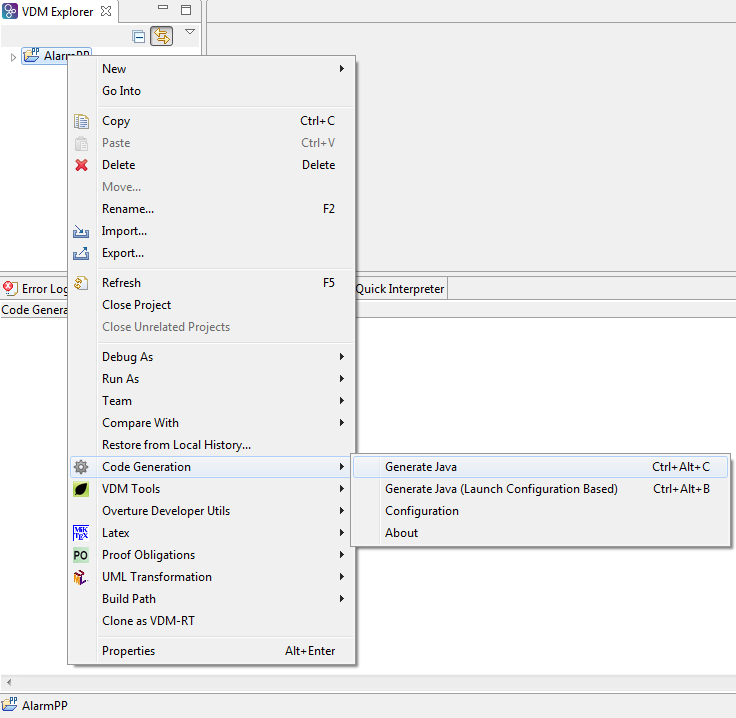
\includegraphics[width=10cm]{screenDumps/javacg_menu}
\caption{Launching the Java code generator.\label{fig:javacg_menu}}
\end{center}
\end{figure}

\begin{figure}[htbp]
\begin{center}
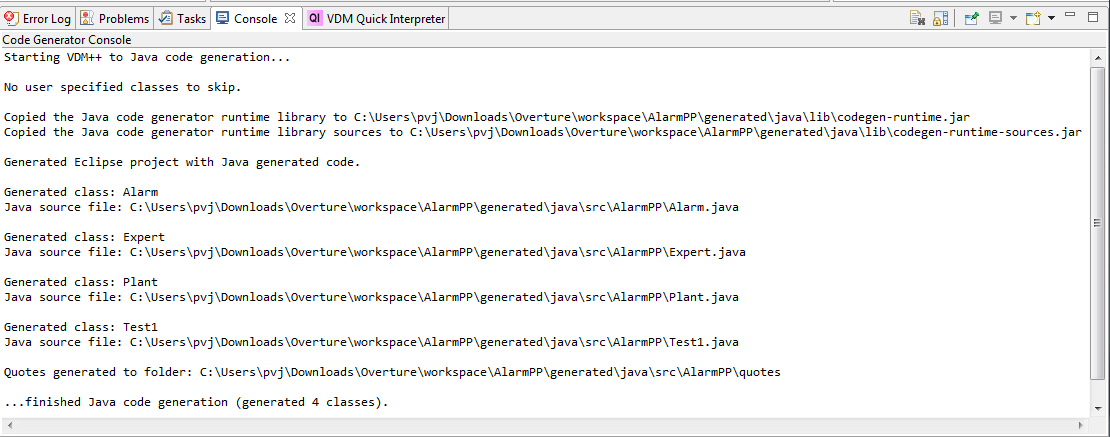
\includegraphics[width=\linewidth]{screenDumps/javacg_output}
\caption{The status of code generating the \texttt{AlarmPP}
example.\label{fig:javacg_output}}
\end{center}
\end{figure}

The Java code generator can be launched via the context menu as shown
in Figure~\ref{fig:javacg_menu}. Alternatively, this can be done by
highlighting the project in the VDM explorer and typing one of the
shortcuts associated to this plugin.\\

\noindent The Java code generator operates in two different modes:

\begin{itemize}

\item \emph{Regular mode:} In this mode the Java code generator
  produces an Eclipse project with all the generated code. Java code
  generation in this mode can also be initiated using the
  \texttt{Ctrl+Alt+C} shortcut.

\item \emph{Launch Configuration mode:}. Is currently limited to
  VDM++. This mode is like regular code generation except that the
  Java code generator also prompts the user for a launch configuration
  as input for the code generation process. Based on this launch
  configuration the Java code generator constructs an entry point (a
  \texttt{main} method really) that serves as an entry point for the
  generated code. Launch configuration based code generation can be
  initiated using the \texttt{Ctrl+Alt+B} shortcut.

\end{itemize}

\noindent Upon completion of the code generation process the status is
output to the console as shown in Figure~\ref{fig:javacg_output}. In
particular this figure shows the status of code generating the
\texttt{AlarmPP} model available in the Overture standard examples. As
indicated by the console output, the generated code is available as an
Eclipse project in the \texttt{<workspace>/<project>/generated/java}
folder.

\noindent The Java code generator is also exposed as a Maven plugin in
order to provide support for build and test automation. In essence
this means that the Java code generator can be invoked from build
environments that use Maven to manage Java projects. This allows code
generated VDM models to be seamlessly integrated with other
dependencies such as manually implemented components that the VDM
model access via the Java bridge (see chapter~\ref{sec:linkToJava}),
user-interfaces or third-party libraries. Another feature of this
Maven plugin is that it allows model tests, written using
\texttt{VDMUnit} to be code generated to JUnit4 tests, which can be
executed via Maven in order to validate the generated code. An online
tutorial that demonstrates how to use the Maven plugin is available
via~\cite{DelegateTutorial}.

\section{Configuration of the Java Code Generator}

The Java code generator can be configured via a preference page as
shown in Figure~\ref{fig:javacg_config}. The preference page can be
accessed in the way you would normally access an Eclipse preference
page or via the context menu shown above in
Figure~\ref{fig:javacg_menu}. The Java code generator provides a few
options that allows the user to configure the code generation process
(see Figure~\ref{fig:javacg_config}). The sub-sections below treat
each of these configuration parameters individually, in the order they
appear in the preference page.

\begin{figure}[htbp]
\begin{center}
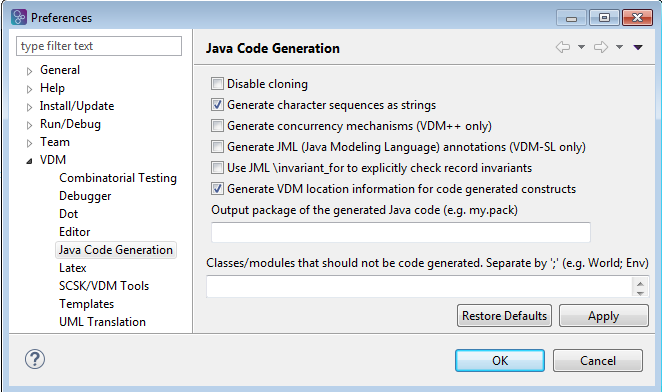
\includegraphics[width=15cm]{screenDumps/javacg_config}
\caption{Configuration of the Java code generator.\label{fig:javacg_config}}
\end{center}
\end{figure}

\subsection{Disable cloning}

In order to respect the value semantics of VDM the Java code generator
sometime needs to perform deep copying of objects that represent
composite value types (records, tuples, tokens, sets, sequences and
maps). For example, in VDM a record is a value type, which means that
occurrences of the record must be copied when it appears in the
right-hand side of an assignment, it is passed as an argument or
returned as a result. However, Java does not support composite value
types like structs and records, and as a consequence record types must
be represented using classes, which use reference semantics. This
means that an object reference, which is used to represent a composite
value type in the generated Java code must be deep copied when it
appears in the right-hand side of an assignment, it is passed as an
argument or returned as a result. For arbitrarily complex value types
(such as records composed of record or sets of composed of sets) deep
copying may introduce a significant overhead in the generated code. If
the specification subject to code generation does not truly rely on
value semantics the user may wish to disable deep copying of value
types in the generated code in order to remove this overhead. The user
should, however, be aware that disabling of cloning may lead to code
being generated that does not preserve the semantics of the input
specification and in general disabling of cloning is discouraged. By
default cloning is enabled.

\subsection{Generate character sequences as strings}
\label{sec:charseqs-as-strings}

In VDM a string is a sequence of characters and there is no notion of
a string type. Java in particular works differently since it uses a
separate type to represent a string. The default behaviour of the Java
code generator is to code generate sequences of characters as strings
and subsequently do the necessary conversion between between strings
and sequences in the generated code. Another possibility is to treat a
string literal for what it truly is, namely a sequence of characters,
and thereby avoid any conversion between strings and sequences. In
order to do that, i.e.\ \textit{not} generating character sequences as
strings, the corresponding option must be unchecked.

\subsection{Generate concurrency mechanisms}

If the user does not rely on the concurrency mechanisms of VDM++ and
does not want to include support for them in the generated code the
corresponding option in the preference page must be unchecked. By
default the behaviour of the Java code generator is to not include
support for the concurrency mechanisms of VDM++ in the generated code.

\subsection{Generate Java Modeling Language (JML) annotations}

When a VDM model is code generated to Java all the contract-based
elements of the model, i.e.\ the pre conditions, post conditions and
invariants, are ignored by default. When this option is selected the
contract-based elements of a VDM-SL model are translated to JML
annotations~\cite{Burdy&05} that are added to the generated Java
code~\cite{Jorgensen&17,Jorgensen&17a}. This allows the system
properties, expressed in terms of pre conditions, post conditions and
invariants, to be checked against the generated code. The generated
JML annotated programs can be checked for corrected using a JML tool
such as OpenJML\footnote{\url{http://www.openjml.org}}. A complete
definition of the JML translation can be found via the the references
provided.\\

\subsection{Use JML \textbackslash invariant\_for to explicitly check record invariants}
\label{sec:inv-for}

The JML generator offers two ways to perform the invariant check of a
record. By default the JML generator does this by invoking a
\texttt{valid} method generated for each record definition. When this
option is enabled the JML generator instead uses the JML
\vdmkw{invariant\_for} construct to perform the record invariant
checks. Note that the \vdmkw{invariant\_for} construct is currently
not supported by OpenJML, which is the reason why this option is not
enabled by default.

\subsection{Generate VDM location information for code generated constructs}
\label{sec:vdm-loc}

When a VDM model is code generated it can be helpful to know where the
constructs in the generated code originate from. When this option is
enabled the Java code generator will generate VDM location information
for methods, statements and local declarations in the generated
code. More specifically, the Java code generator will generate a Java
source code comment containing the name of the VDM source file and the
line number and the position, for each method, statement and local
declaration. As an example, the code fragment below says that the Java
return statement originates from a VDM construct at line 25,
position 12 in \texttt{File.vdmsl}.\\

\noindent \texttt{/* File.vdmsl 25:12 */\\return 42;}

\subsection{Choose output package}
\label{sec:javapackage}

The Java code generator allows the output package of the generated
code to be specified. If the user does not specify a package, the code
generator outputs the generated Java code to a package with the same
name as the VDM project. If the name of the project is not a valid
java package, then the generated code is output to the default Java
package.

\subsection{Skip classes/modules during the code generation process}

It may not always make sense to code generate every class or module in
a VDM project. A class or module can often be skipped if it acts as an
execution entry point or it is used to load input for the
specification. Classes or modules that the user wants to skip can be
specified in the text box in the Java code generator preference page
by separating the class/module names by a semicolon. As an example,
\texttt{World;Env} makes the code generator skip code generation of
\texttt{World} and \texttt{Env}, while generating code for any other
module or class. For convenience the output of the Java code generator
will also inform the user about what classes or modules are being
skipped.

\section{Limitations of the Java Code Generator}

If the Java code generator encounters a construct that it cannot code
generate it will report it as unsupported to the user and the user can
then try to rewrite that part of the specification using other
(supported) constructs. Reporting of unsupported constructs is done
via the console output and using editor markers. In order to
demonstrate this, Figure~\ref{fig:javacg_unsupported} shows the
console output of the Java code generator when it encounters a type
bind, which is an example of an unsupported language construct. Note
the small marker appearing in the editor in order to point out where
use of the construct appears. For the type bind example in
Figure~\ref{fig:javacg_unsupported} the following message is reported:\\

\noindent \texttt{Following VDM constructs are not supported by the
  code generator:\\ b:(bool * bool) (ATypeMultipleBind) at
  6:14. Reason:\\ Type binds are not supported}\\

\begin{figure}[htbp]
\begin{center}
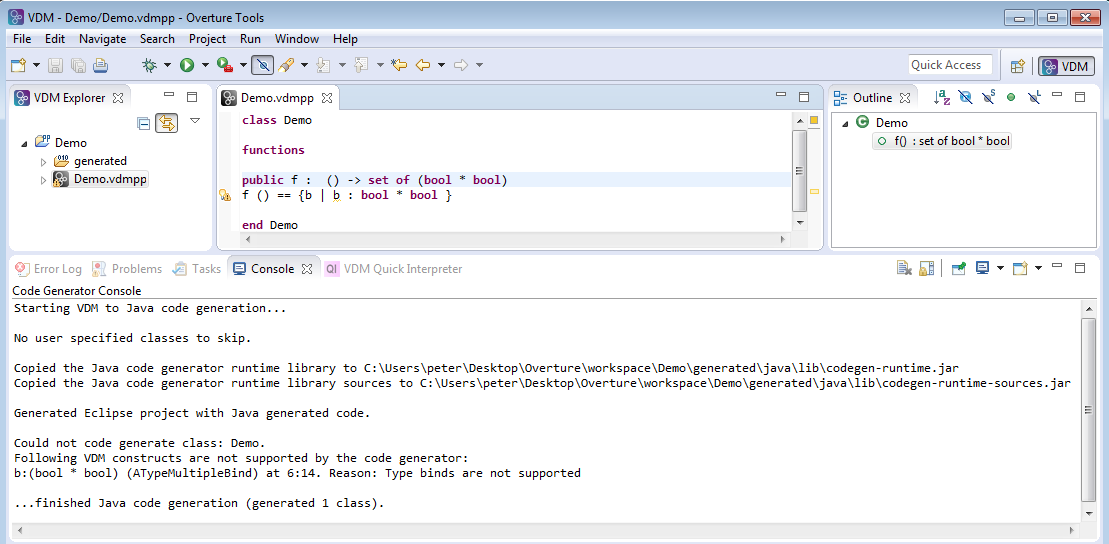
\includegraphics[width=\linewidth]{screenDumps/javacg_unsupported}
\caption{Reporting of unsupported constructs in the
console.\label{fig:javacg_unsupported}}
\end{center}
\end{figure}

The user will get similar messages and markers for other unsupported
VDM constructs. To summarise, the Java code generator currently does
not support code generation of multiple inheritance and neither does
it support traces, type binds, invariant checks and pre and post
conditions. Furthermore, let expressions appearing on the right-hand
side of an assignment will also be reported as unsupported. The Java
code generator also does not support every pattern. The patterns that
are currently not supported are: object, map union, map, union, set,
sequence, concatenation and match value.

\section{The Code Generation Runtime Library}

The generated code relies on a runtime library used to represent some
of the types available in VDM (tokens, tuples etc.) as well as
collections and support for some of the complex operators such as
sequence modifications. For simplicity every Eclipse project generated
by the Java code generator contains the runtime library. More
specifically, there is a copy of the runtime library containing only
the binaries (\texttt{lib/codegen-runtime.jar}) as well as a version
of the runtime library that has the source code attached
(\texttt{lib/codegen-runtime-sources.jar}). The runtime library is
imported by every code generated class using the Java import statement
\texttt{\textbf{import} org.overture.codegen.runtime.*;} and in order
to compile the generated Java code the runtime library must be visible
to the Java compiler.

Similar to VDMTools the runtime library also provides implementation
for subset of the functionality available in the standard libraries:
The runtime library provides a full implementation of the
\texttt{MATH} library, support for conversion of values into character
sequences as provided by the \texttt{VDMUtil}, and finally
functionality to write to the console as available in the \texttt{IO}
library.

\section{Translation of the VDM types and type constructors}
\label{sec:type-mappings}

Table ~\ref{tbl:type-mappings} describes how the VDM type(s) in the
left column are represented in the generated Java code (the right
column). In this table \texttt{pack} is the user-specified root
package of the generated Java code (see section \ref{sec:javapackage})
and \texttt{E}, \texttt{D} and \texttt{R} represent arbitrary VDM
types. The type mapping in the last row is only used when the
\emph{Generate character sequences as strings} option is selected (see
section \ref{sec:charseqs-as-strings}). Some of the types used to
represent the VDM types are native Java types (from package
\texttt{java.lang}), others are part of the Java code generator
runtime library (from package \texttt{org.overture.codegen.runtime}),
and some are generated.

\begin{center}
    \begin{tabular}{| l | l |}
    \hline
    VDM type(s) & Java type \\ \hline
    \vdmkw{bool} & \texttt{java.lang.Boolean} \\ \hline
    \vdmkw{nat}, \vdmkw{nat1}, \vdmkw{int}, \vdmkw{rat}, \vdmkw{real} & \texttt{java.lang.Number} \\ \hline
    \vdmkw{char} & \texttt{java.lang.Character} \\ \hline
    \vdmkw{token} & \texttt{org.overture.codegen.runtime.Token} \\ \hline
    Tuple types (e.g.\ \vdmkw{nat} \texttt{*} \vdmkw{nat}) & \texttt{org.overture.codegen.runtime.Tuple} \\ \hline
    Union types (e.g.\ \vdmkw{nat} \texttt{|} \vdmkw{nat}) & \texttt{java.lang.Object} \\ \hline
    Quote type \texttt{ <T>} & \texttt{pack.quotes.TQuote} \\ \hline
    User-defined types \texttt{T = D} & Represented using the representation of type \texttt{D} \\ \hline
    A class \texttt{C} & \texttt{pack.C} \\ \hline
    Record type \texttt{R} defined in class or module \texttt{M} & Inner class \texttt{pack.M.R}  \\ \hline
    \vdmkw{set of} \texttt{ E} & \texttt{org.overture.codegen.runtime.VDMSet} \\  \hline
    \vdmkw{map} \texttt{ D } \vdmkw{to} \texttt{ R}, \vdmkw{inmap} \texttt{ D } \vdmkw{to} \texttt{ R} & \texttt{org.overture.codegen.runtime.VDMMap} \\  \hline
    \vdmkw{seq of} \texttt{ E}, \vdmkw{seq1 of} \texttt{ E}  & \texttt{org.overture.codegen.runtime.VDMSeq} \\  \hline
    \vdmkw{seq of char}, \vdmkw{seq1 of char} & \texttt{java.lang.String} \\  \hline
    \end{tabular}
  \captionof{table}{The type mappings used by the Java code generator.}
  \label{tbl:type-mappings}
\end{center}
%
%
%
\section{The C Code Generator}
Translation of VDM models to C code is a new feature of Overture.
%
The target language of the C generator is the executable subset of VDM-RT.
%
It is not yet feature-complete, but it can handle models that do not use sophisticated features of VDM-RT.

In this section we give an overview of the current state of language feature support.
%
The translation strategy is then described in some detail as a means of providing a tutorial introduction to calling into the generated model.
%
%
%
\subsection{Language Feature Support Status}
Overture's C code generator is under active development.
%
At present, items in black are tested and known, to the best of the developers' knowledge, to translate correctly to C.
%
Items in \textcolor{red}{red} are not yet supported.
%
\begin{itemize}
%
\item  Classes.
%
\item  Inheritance.
%
\item  Overloading and overriding.
%
\item  Nested constructor calling.
%
\item  The \texttt{self} expression.
%
\item  Type definitions.
\begin{itemize}
\item  \textcolor{red}{Type invariants}.
\end{itemize}
%
\item  Boolean and numeric expressions.
\begin{itemize}
\item  \textcolor{red}{Quantifiers}.
\end{itemize}
%
\item  Let expressions.
%
\item  \texttt{is\_(\textit{var}, \textit{type})} testing for basic types.
%
\item  Records.
%
\item  Products.
%
\item  Sets, sequences and maps.
\begin{itemize}
\item  \textcolor{red}{Nested state designators, \emph{e.\@g.\@} \texttt{a(i)(j) := k}}.
\end{itemize}
%
\item  Explicit functions and operations.
\begin{itemize}
\item  \textcolor{red}{Lambda abstractions}.
\item  \textcolor{red}{Pre-\@ and post-conditions}.
\end{itemize}
%
\item  Loops.
\begin{itemize}
\item  For index loops.
\item  While loops.
\end{itemize}

%
\item  \textcolor{red}{Real-time and distribution features}.
\begin{itemize}
\item  The \verb|time| statement.
\end{itemize}
%
\item  I/O library.
\begin{itemize}
\item  \textcolor{red}{String patterns}.
\item  \textcolor{red}{General file I/O}.
\end{itemize}
%
\item \textcolor{red}{CSV library}.
\begin{itemize}
\item  flinecount()
\item  freadval~[~seq of real~]~()
\end{itemize}
%
\item MATH library.
\begin{itemize}
\item  \textcolor{red}{rand()}
\item  \textcolor{red}{srand()}
\item  \textcolor{red}{srand2()}
\end{itemize}
%
\end{itemize}

Like the Java code generator, the C code generator can be invoked from the context menu in the VDM project explorer, as shown in in Figure \ref{fig:invoking}.
%
%
%
\begin{figure}[ht]
\centering
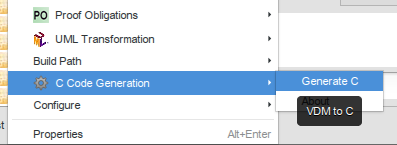
\includegraphics[width=3.7in]{figures/InvokingCCG.png}
\caption{Invoking the C code generator.}
\label{fig:invoking}
\end{figure}
%
%
%
Unlike the Java code generator, it must be installed through Overture's ``Install New Software \dots'' feature.
%
The repository URL is
%
%
%
\begin{quote}
\url{http://overture.au.dk/vdm2c/master/repository/}.
\end{quote}
%
Code is emitted to the folder \texttt{generated/src/c} under the corresponding VDM project.
%
Please note that this folder is wiped clean each time code is generated.
%
Additional development work on the generated code \emph{must not} be carried out in this folder.

The generator will emit a \texttt{main.c} file containing a skeletal \texttt{main()} function.
%
The body of this function contains calls to initialize and shutdown the garbage collector used to manage memory usage in the generated code.
%
The garbage collector is not invoked automatically.
%
It is therefore necessary to insert calls to the function \texttt{vdm\_gc()} in order to do so.
%
It is safe to insert calls to reclaim unused memory inside code developed by hand, for instance after every execution of a periodic task, but it is generally unsafe to modify the generated code to do so.
%
The \texttt{main.c} file also contains helper functions for system-wide initialization and tear-down of model \texttt{values} and static fields.
%
The implementation of these is discussed below.
%
The generator also emits a CMake file called \texttt{Project}\-\texttt{CMake}\-\texttt{Lists.txt}.
%
When renamed to \texttt{CMake}\-\texttt{Lists.txt}, executing
%
%
%
\begin{quote}
\texttt{cmake .}\\
\texttt{make}
\end{quote}
%
%
%
in the generated code root directory will compile an executable, but inert, binary of the generated model.
%
At this point the user is free to populate the \texttt{main()} function.
%
The header file \texttt{Mangled}\-\texttt{Names.h} contains the correspondences between model identifiers and the mangled names used internally in the generated code.
%
This file can be used to call into the generated model using approximately the naming convention of the VDM model.
%
%
%
\subsection{The C Translation Strategy}
The priority of the translation strategy is to remain faithful to the VDM-RT semantics described above.
%
The strategy therefore assumes that VDM-RT specifications have been validated using Overture's various facilities.
%
This section describes the strategy and the two sides of the translation mechanism, the implementation of the strategy and the native C support library.
%
The generated code can be compiled and executed by means of a CMake build mechanism and an empty \texttt{main.c} file, but no calls into the generated code proper are made.
%
%
%
%\paragraph{Executable VDM}
%\revisit{What is, but focus on what is not, executable.}
%
%
%
\subsubsection{Native Support Library}
Implementations generated from VDM-RT models consist of two parts, the generated code and a native support library\footnote{The design of the native library is based on the following four sources:\\\url{http://www.pvv.ntnu.no/~hakonhal/main.cgi/c/classes/}, accessed 2016-09-22.\\\url{http://www.eventhelix.com/RealtimeMantra/basics/}\\\parbox{1cm}{~}\url{ComparingCPPAndCPerformance2.htm}, accessed 2016-09-22.\\\url{http://www.go4expert.com/articles/}\\\parbox{1cm}{~}\url{virtual-table-vptr-multiple-inheritance-t16616/}, accessed 2016-09-22.\\\url{http://www.go4expert.com/articles/virtual-table-vptr-t16544/}, accessed 2016-09-22.}.
%
The native library is fixed and does not change during the code generation process.
%
We illustrate its design here by means of very simple generated VDM models.

The native library provides a single fundamental data structure in support of all the VDM-RT data types, called \texttt{TypedValue}.
%
The complete definition is shown in Listing \ref{lst:tvp}.
%
A pointer to \texttt{TypedValue} is \texttt{\#define}d as \texttt{TVP}, and is used throughout the implementation.
%
%
%
\begin{lstlisting}[language=C,caption={Fundamental code generator data type.},label={lst:tvp},frame=tlbr]{lst:vdmtype}
typedef enum {
	VDM_INT, VDM_NAT, VDM_NAT1, VDM_BOOL, VDM_REAL, 
	VDM_RAT, VDM_CHAR, VDM_SET, VDM_SEQ, VDM_MAP,
	VDM_PRODUCT, VDM_QUOTE, VDM_RECORD, VDM_CLASS
} vdmtype;

typedef union TypedValueType {
	void* ptr;			// VDM_SET, VDM_SEQ, VDM_CLASS,
	            			// VDM_MAP, VDM_PRODUCT
	int intVal;			// VDM_INT and INT1
	bool boolVal;			// VDM_BOOL
	double doubleVal;		// VDM_REAL
	char charVal;			// VDM_CHAR
	unsigned int uintVal;		// VDM_QUOTE
} TypedValueType;

struct TypedValue {
	vdmtype type;
	TypedValueType value;
};

struct Collection {
	struct TypedValue** value;
	int size;
};
\end{lstlisting}
%
%
%
An element of this type carries information about the type of the VDM value represented and the value proper.
%
For space efficiency, the value storage mechanism is a C \texttt{union}.

Members of the basic, unstructured types \texttt{int}, \texttt{char}, \emph{etc.}\@ are stored directly as values in corresponding fields.
%
Due to subtype relationships between certain VDM types, for instance \texttt{nat} and \texttt{nat1}, fields in the union can be reused.
%
Functions to construct such basic values are provided:
%
%
%
\begin{itemize}
\item \texttt{TVP newInt(int)}
\item \texttt{TVP newBool(bool)}
\item \texttt{TVP newQuote(unsigned int)}
\item \emph{etc.\@}
\end{itemize}
%
%
%
All the operations defined by the VDM language manual on basic types are implemented one-to-one.
%
They can be found in the header file\\\texttt{VdmBasicTypes.h}.

Members of structured VDM types, such as \texttt{seq} and \texttt{set}, are stored as references, owing to their variable size.
%
The \texttt{ptr} field is dedicated to these.
%
These collections are represented as arrays of \texttt{TypedValue} elements, wrapped in the C structure \texttt{Collection}.
%
The field \texttt{size} of \texttt{Collection} records the number of elements in the collection.
%
Naturally, collections can be nested.
%
At the level of VDM these data types are immutable and follow value semantics.
%
But internally they are constructed in various ways.
%
For instance, internally creating a fresh set from known values is different from constructing one value by value according to some filter on values.
%
In the former case a new set is created in one shot, whereas in the latter an empty set is created to which values are added.
%
Several functions are provided for constructing collections which accommodate these different situations.
%
%
%
\begin{itemize}
\item \texttt{newSetVar(size\_t, ...)}
\item \texttt{newSetWithValues(size\_t, TVP*)}
\item \texttt{newSeqWithValues(size\_t, TVP*)}
\item \emph{etc.\@}
\end{itemize}

These rely on two functions for constructing the inner collections of type \texttt{struct Collection} at field \texttt{ptr}:
%
%
%
\begin{itemize}
\item \texttt{TVP newCollection(size\_t, vdmtype)}
\item \texttt{TVP newCollectionWithValues(size\_t, vdmtype, TVP*)}
\end{itemize}
%
%
%
The former creates an empty collection that can be grown as needed by memory re-allocation.
%
The latter wraps an array of values for inclusion in a \texttt{TVP} value of structured type.
%
All the operations defined in the VDM language manual on structured types are implemented one-to-one.
%
They can be found in the header files \texttt{VdmSet.h}, \texttt{VdmSeq.h} and \texttt{VdmMap.h}.
%
%The functions implementing the operations defined in the VDM language manual \ref{} on basic and structured types are listed in Table \ref{}.
%
%

%\begin{tabular}{l|l|l}
%\textbf{Category} & \textbf{VDM Operation} & \textbf{Native Library Operation}\\
%\hline\\
%Basic type & & \\
%\hline\\
%Set & & \texttt{vdmSetMemberOf}\\
%\hline\\
%Sequence & & \\
%\hline\\
%Map & &
%\end{tabular}
%
VDM's object orientation features are fundamentally implemented in the native library using C \texttt{struct}s.
%
In brief, a class is represented by a \texttt{struct} whose fields represent the fields of the class.
%
The functions and operations of the class are implemented as functions associated with the corresponding \texttt{struct}.

Consider the following example VDM specification.
%
%
%
\begin{lstlisting}[language=VDM++,caption={Example VDM model.},label={lst:vdmexample},frame=tlbr]{lst:vdmexample}
class A
instance variables
	private i : int := 1;

operations
	public op : () ==> int
	op() ==
		return i;
end A
\end{lstlisting}
%
%
%
The code generator produces the two files \texttt{A.h} and \texttt{A.c}, shown below.
%
%
%
\begin{lstlisting}[language=C,caption={Corresponding header file \texttt{A.h}.},label={lst:vdmexheader},frame=tlbr]{lst:vdmexheader}
#include "Vdm.h"
#include "A.h"

#define CLASS_ID_A_ID 0

#define ACLASS struct A*

#define CLASS_A__Z2opEV 0

struct A
{
	VDM_CLASS_BASE_DEFINITIONS(A);
	 
	VDM_CLASS_FIELD_DEFINITION(A,i);
	
};

TVP _Z1AEV(ACLASS this_);

ACLASS A_Constructor(ACLASS);

\end{lstlisting}
%
%
%
The basic construct is a \texttt{struct} containing the class fields and the class virtual function table:
%
%
%
\begin{lstlisting}[language=C,caption={Macro for defining class virtual function tables.},label={lst:virttablmacro},frame=tlbr]{lst:virttablmacro}
#define VDM_CLASS_FIELD_DEFINITION(className, name) \
	TVP m_##className##_##name
	
#define VDM_CLASS_BASE_DEFINITIONS(className) \
	struct VTable * _##className##_pVTable; \
	int _##className##_id; \
	unsigned int _##className##_refs
\end{lstlisting}
%
%
%
The virtual function table contains information necessary for resolving a function call in a multiple inheritance context as well as a field which receives a pointer to the implementation of the operation \texttt{op}.
%
%
%
\begin{lstlisting}[language=C,caption={Virtual function table.},label={lst:virttablmacro},frame=tlbr]{lst:virttabl}
typedef TVP (*VirtualFunctionPointer)(void * self, ...);

struct VTable
{
	//Fields used in the case of multiple inheritance.
	int d;
	int i;
	
	VirtualFunctionPointer pFunc;
};
\end{lstlisting}
%
%
%
The rest of the important parts of the implementation consists of the function implementing \texttt{op()}, the definition of the virtual function table into which this slots and the complete constructor mechanism.
%
%
%
\begin{lstlisting}[language=C,caption={Corresponding implementation file \texttt{A.c}.},label={lst:vdmeximpl},frame=tlbr]{lst:vdmeximpl}
#include "A.h"
#include <stdio.h>
#include <string.h>

void A_free_fields(struct A *this)
{
	vdmFree(this->m_A_i);
}

static void A_free(struct A *this)
{
	--this->_A_refs;
	if (this->_A_refs < 1)
	{
		A_free_fields(this);
		free(this);
	}
}
 
/* A.vdmrt 6:9 */
static  TVP _Z2opEV(ACLASS this)
{
	/* A.vdmrt 8:10 */
	TVP ret_1 = vdmClone(newBool(true));

	/* A.vdmrt 8:3 */
	return ret_1;
}


static struct VTable VTableArrayForA [] =
{
	{0,0,((VirtualFunctionPointer) _Z2opEV),},
};
 

ACLASS A_Constructor(ACLASS this_ptr)
{
	if(this_ptr==NULL)
	{
		this_ptr = (ACLASS) malloc(sizeof(struct A));
	}

	if(this_ptr!=NULL)
	{
		this_ptr->_A_id = CLASS_ID_A_ID;
		this_ptr->_A_refs = 0;
		this_ptr->_A_pVTable=VTableArrayForA;

		this_ptr->m_A_i= NULL ;
	}

	return this_ptr;
}

// Method for creating new "class"
static TVP new()
{
	ACLASS ptr=A_Constructor(NULL);

	return newTypeValue(VDM_CLASS,
		(TypedValueType)
			{.ptr=newClassValue(ptr->_A_id,
				&ptr->_A_refs,
				(freeVdmClassFunction)&A_free,
				ptr)});
}
 

/* A.vdmrt 1:7 */
TVP _Z1AEV(ACLASS this)
{
	TVP __buf = NULL;

	if(this == NULL)
	{
		__buf = new();

		this = TO_CLASS_PTR(__buf, A);
	}

	return __buf;
}
\end{lstlisting}
%
%
%
\texttt{TO\_CLASS\_PTR} merely unwraps values and can be ignored for now.

Construction of an instance of class \texttt{A} starts with a call to \texttt{\_Z1AEV}.
%
An instance of \texttt{struct A} is allocated and its virtual function table is populated with the pointer to the implementation of \texttt{op()}, \texttt{\_Z2opEV}.
%
The latter name is a result of a name mangling scheme implemented in order to avoid name clashes in the presence of inheritance\footnote{The name mangling scheme is based on the following sources:\\\url{https://en.wikipedia.org/wiki/Name_mangling}, accessed 2016-09-28.\\\url{http://www.avabodh.com/cxxin/namemangling.html}, accessed 2016-09-28.}.
%
A header file called \texttt{MangledNames.h} provides the mappings between VDM model identifiers and mangled names in the generated code.
%
This mapping aids in writing the \texttt{main} function.
%
The scheme used is \texttt{ClassName\_identifier}.
%
Listing \ref{lst:manglednames} shows the contents of the file for the example model.
%
%
%
\begin{lstlisting}[language=C,caption={File \texttt{MangledNames.h}.},label={lst:manglednames},frame=tlbr]{lst:manglednames}
#define A_op _Z2opEV
#define A_A _Z1AEV
\end{lstlisting}
%
%
%

By default, the code generation process provides an empty \texttt{main.c} file such that it is possible to compile the generated code initially.
%
It will, of course, be completely inert.
%
The following example populated \texttt{main.c} file illustrates how to make use of the generated code.
%
%
%
\begin{lstlisting}[language=C,caption={Example \texttt{main.c} file.},label={lst:mainexample},frame=tlbr]{lst:mainexample}
#include "A.h"

int main()
{
	TVP a_instance = _Z1AEV(NULL);
	TVP result;
	
	result = CALL_FUNC(A, A, a_instance, CLASS_A__Z2opEV);
	
	printf("Operation op returns:  %d\n", result->value.intVal);
	
	vdmFree(result);
	vdmFree(a_instance);
	
	return 0;
}
\end{lstlisting}
%
%
%
Had the class \texttt{A} contained any \texttt{value}s or \texttt{static} fields, the very first calls into the model would have been to \texttt{A\_\allowbreak{}const\_\allowbreak{}init()} and \texttt{A\_\allowbreak{}static\_\allowbreak{}init()}.
%
As this is not the case here, an instance of the class implementation is first created, together with a variable to store the result of \texttt{op}.
%
The macro \texttt{CALL\_FUNC} carries out the necessary calculations for calling the correct version of \texttt{\_Z2opEV} in the presence of inheritance and overriding (not the case here).
%
%
%
\begin{lstlisting}[language=C,caption={Macros supporting function calls.},label={lst:fncallmacros},frame=tlbr]{lst:fncallmacros}
#define GET_STRUCT_FIELD(tname,ptr,fieldtype,fieldname) \
	(*((fieldtype*)(((unsigned char*)ptr) + \
			offsetof(struct tname, fieldname))))


#define GET_VTABLE_FUNC(thisTypeName,funcTname,ptr,id) \
	GET_STRUCT_FIELD(thisTypeName,ptr,struct VTable*, \
			_##funcTname##_pVTable)[id].pFunc


#define CALL_FUNC(thisTypeName,funcTname,classValue,id, args... ) \
	GET_VTABLE_FUNC( thisTypeName, \
			funcTname, \
			TO_CLASS_PTR(classValue,thisTypeName), \
			id) \
	(CLASS_CAST(TO_CLASS_PTR(classValue,thisTypeName), \
		thisTypeName, \
		funcTname), ## args)
\end{lstlisting}
%
%
%
The result is assigned to \texttt{result}, which is then accessed according to the structure of \texttt{TVP}.
%
The function \texttt{vdmFree} is the main memory cleanup function for variables of type \texttt{TVP}.
%
%
%
\subsubsection{Translating Features of VDM-SL}
In this section we discuss how the basic features of VDM-RT, those contained in the subset VDM-SL, are translated to C.
%
\paragraph{Basic data types}
Instances of the fundamental data types of VDM-SL (integers, reals, characters \emph{etc}.\@) translate directly to instances of type \texttt{TVP} with the appropriate field of the union structure \texttt{TypedValueType} set to the value of the instance.
%
They are instantiated using the corresponding constructor functions \texttt{newInt()}, \texttt{newBool()} \emph{etc}.\@ introduced above.
%
Operations on fundamental data types preserve value semantics by always allocating new memory for the result \texttt{TVP} instance and returning the corresponding pointer.
%
\paragraph{Structured types.}
Like basic types, aggregate types such as sets and maps are treated in exactly the same way.
%
The support library provides both the data type infrastructure as well as the operations on aggregate types such that translation is rendered straightforward.
%
For example, the expression
%
%
%
\begin{lstlisting}[language=VDM++,frame=tlbr]
a : set of int := {1} union {2}
\end{lstlisting}
%
%
%
translates directly to 
%
%
%
\begin{lstlisting}[language=C,frame=tlbr]
TVP a = vdmSetUnion(newSetVar(1, newInt(1)), newSetVar(1, newInt(2)));
\end{lstlisting}
%
%
%
where \texttt{newSetVar()} is one of the several special-purpose internal constructors.
%
The translation strategy is similar for sequences and maps.
%
Value semantics for these immutable data types is maintained in the same way as for the basic data types.
%
%
%
\paragraph{Quote types}
Quote types such as that shown in Listing \ref{lst:quoteex} are treated at the individual element level.
%
Each element is assigned a unique number via a \texttt{\#define} directive, as shown in Listing \ref{lst:quoteex}.
%
%
%
\begin{lstlisting}[language=VDM++,caption={Quote type example.},label={lst:quoteex},frame=tlbr]{lst:quoteex}
class QuoteExample

types

	public QuoteType = <Val1> | <Val2> | <Val3>

end QuoteExample
\end{lstlisting}
%
%
%
\begin{lstlisting}[language=VDM++,caption={Quote type example translation.},label={lst:quoteimpl},frame=tlbr]{lst:quoteimpl}
...

#ifndef QUOTE_VAL1
#define QUOTE_VAL1 2658640
#endif /* QUOTE_VAL1 */

#ifndef QUOTE_VAL2
#define QUOTE_VAL2 2658641
#endif /* QUOTE_VAL2 */

...
\end{lstlisting}
%
%
%
\paragraph{Union types.}
The decision to keep run-time type information for every variable of type \texttt{TVP} obviates the need for a translation strategy for union types.
%
%
%
\subsubsection{Translating Features of VDM++}
\paragraph{Classes}
%
Earlier we introduced the mechnism of C structures used to represent classes.
%
Translation of a model class is therefore straightforward, with each class receiving its own specific \texttt{struct}.
%
As illustrated in Listings \ref{lst:vdmexheader} and \ref{lst:vdmeximpl} above, each class receives its own pair of C header and implementation files.
%
Most importantly, the header file contains the definition of the corresponding class \texttt{struct} and the declarations of the interface functions for this struct.
%
These include the top-level constructor and initialization and cleanup functions for class \texttt{values} and \texttt{static} field declarations.
%
The implementation (\texttt{.c}) file contains the constructor mechanism, the definition of the virtual function table of the class and the implementations of the class's functions and operations.
%
The virtual function table is constructed in accordance with the inheritance hierarchy in which the class belongs (this is discussed below).
%
Class \texttt{values} definitions and static fields are implemented as global variables.
%
Their definitions are also inserted in the implementation file, along with initializer and cleanup functions to be called, respectively, when the implementation starts and terminates.

\paragraph{Inheritance}
%
The effect of inheritance is to augment the definition of the inheriting class with the features of the parent class, \emph{modulo} overriding.
%
In our \texttt{struct}-based implementation of classes and objects, the traits of the base class are copied into the \texttt{struct} corresponding to the inheriting class.
%
Therefore, the \texttt{struct} of the inheriting class duplicates the fields and virtual function table of the base class.

Consider the translation of the following model with inheritance.
%
Despite its cumbersome length, we provide the listing of the complete translation so that the reader may also gain familiarity (at his/her own pace) with all the elements of the generated code.
%
%
%
\begin{lstlisting}[language=VDM++,frame=tlbr]
class A
instance variables
public field_A : int := 0;

operations
public opA : int ==> int
opA(i) == return i;
end A


class B is subclass of A
operations
public opB : () ==> ()
opB() == skip;
end B


class C
instance variables
b : B := new B();

operations
public op : () ==> int
op() == return b.opA(b.field_A);
end C
\end{lstlisting}
%
%
%
The six files \texttt{A.h}, \texttt{A.c}, \texttt{B.h}, \texttt{B.c}, \texttt{C.h} and \texttt{C.c} reproduced below make up the complete translation.
%
%
%
\begin{lstlisting}[language=C,frame=tlbr,caption="File A.h."]
// The template for class header
#ifndef CLASSES_A_H_
#define CLASSES_A_H_

#define VDM_CG

#include "Vdm.h"

//include types used in the class
#include "A.h"


extern TVP numFields_1;

#define CLASS_ID_A_ID 0
#define ACLASS struct A*

#define CLASS_A__Z3opAEI 0

struct A
{
	VDM_CLASS_BASE_DEFINITIONS(A);

	VDM_CLASS_FIELD_DEFINITION(A,field_A);
	VDM_CLASS_FIELD_DEFINITION(A,numFields);
};

TVP _Z1AEV(ACLASS this_);

void A_const_init();
void A_const_shutdown();
void A_static_init();
void A_static_shutdown();

void A_free_fields(ACLASS);
ACLASS A_Constructor(ACLASS);

#endif /* CLASSES_A_H_ */

\end{lstlisting}
%
%
%
\begin{lstlisting}[language=C,frame=tlbr,caption="File A.c."]
#include "A.h"
#include <stdio.h>
#include <string.h>


void A_free_fields(struct A *this)
{
	vdmFree(this->m_A_field_A);
}

static void A_free(struct A *this)
{
	--this->_A_refs;
	if (this->_A_refs < 1)
	{
		A_free_fields(this);
		free(this);
	}
}

static  TVP _Z17fieldInitializer2EV(){
	TVP ret_1 = vdmClone(newInt(0));

	return ret_1;
}

static  TVP _Z17fieldInitializer1EV(){
	TVP ret_2 = vdmClone(newInt(1));

	return ret_2;
}

static  TVP _Z3opAEI(ACLASS this, TVP i){
	TVP ret_3 = vdmClone(i);

	return ret_3;
}

void A_const_init(){
	numFields_1 = _Z17fieldInitializer1EV();

	return ;
}

void A_const_shutdown(){
	vdmFree(numFields_1);

	return ;
}

void A_static_init(){

	return ;
}

void A_static_shutdown(){

	return ;
}

static  struct VTable VTableArrayForA  [] ={

		{0,0,((VirtualFunctionPointer) _Z3opAEI),},
}  ;

ACLASS A_Constructor(ACLASS this_ptr)
{
	if(this_ptr==NULL)
	{
		this_ptr = (ACLASS) malloc(sizeof(struct A));
	}

	if(this_ptr!=NULL)
	{
		this_ptr->_A_id = CLASS_ID_A_ID;
		this_ptr->_A_refs = 0;
		this_ptr->_A_pVTable=VTableArrayForA;

		this_ptr->m_A_field_A= _Z17fieldInitializer2EV();
	}

	return this_ptr;
}

static TVP new(){
	ACLASS ptr=A_Constructor(NULL);

	return newTypeValue(VDM_CLASS, (TypedValueType)
			{	.ptr=newClassValue(ptr->_A_id, &ptr->_A_refs,\
				(freeVdmClassFunction)&A_free, ptr)});
}

TVP _Z1AEV(ACLASS this){
	TVP __buf = NULL;

	if ( this == NULL )
	{
		__buf = new();

		this = TO_CLASS_PTR(__buf, A);
	}

	return __buf;
}

TVP numFields_1 =  NULL ;

\end{lstlisting}
%
%
%
\begin{lstlisting}[language=C,frame=tlbr,caption="File B.h."]
#ifndef CLASSES_B_H_
#define CLASSES_B_H_

#define VDM_CG

#include "Vdm.h"
#include "A.h"
#include "B.h"

#define CLASS_ID_B_ID 1

#define BCLASS struct B*

#define CLASS_B__Z3opBEV 0

struct B
{
	VDM_CLASS_BASE_DEFINITIONS(A);

	VDM_CLASS_FIELD_DEFINITION(A,field_A);
	VDM_CLASS_FIELD_DEFINITION(A,numFields);

	VDM_CLASS_BASE_DEFINITIONS(B);

	VDM_CLASS_FIELD_DEFINITION(B,numFields);
};

TVP _Z1BEV(BCLASS this_);

void B_const_init();
void B_const_shutdown();
void B_static_init();
void B_static_shutdown();

void B_free_fields(BCLASS);
BCLASS B_Constructor(BCLASS);

#endif /* CLASSES_B_H_ */

\end{lstlisting}
%
%
%
\begin{lstlisting}[language=C,frame=tlbr,caption="File B.c."]
#include "B.h"
#include <stdio.h>
#include <string.h>

void B_free_fields(struct B *this)
{
}

static void B_free(struct B *this)
{
	--this->_B_refs;
	if (this->_B_refs < 1)
	{
		B_free_fields(this);
		free(this);
	}
}

static  void _Z3opBEV(BCLASS this){
	{
		//Skip
	};
}

void B_const_init(){
	return ;
}

void B_const_shutdown(){
	return ;
}

void B_static_init(){
	return ;
}

void B_static_shutdown(){
	return ;
}

static  struct VTable VTableArrayForB  [] ={

		{0,0,((VirtualFunctionPointer) _Z3opBEV),},
}  ;

BCLASS B_Constructor(BCLASS this_ptr)
{
	if(this_ptr==NULL)
	{
		this_ptr = (BCLASS) malloc(sizeof(struct B));
	}

	if(this_ptr!=NULL)
	{
		A_Constructor((ACLASS)CLASS_CAST(this_ptr,B,A));

		this_ptr->_B_id = CLASS_ID_B_ID;
		this_ptr->_B_refs = 0;
		this_ptr->_B_pVTable=VTableArrayForB;
	}

	return this_ptr;
}

static TVP new(){
	BCLASS ptr=B_Constructor(NULL);

	return newTypeValue(VDM_CLASS, (TypedValueType)
			{	.ptr=newClassValue(ptr->_B_id, &ptr->_B_refs,\
					(freeVdmClassFunction)&B_free, ptr)});
}

TVP _Z1BEV(BCLASS this){
	TVP __buf = NULL;

	if ( this == NULL )
	{
		__buf = new();
		this = TO_CLASS_PTR(__buf, B);
	}

	_Z1AEV(((ACLASS) CLASS_CAST(this, B, A)));

	return __buf;
}

\end{lstlisting}
%
%
%
\begin{lstlisting}[language=C,frame=tlbr,caption="File C.h."]
#ifndef CLASSES_C_H_
#define CLASSES_C_H_

#define VDM_CG

#include "Vdm.h"
#include "B.h"
#include "C.h"

extern TVP numFields_2;

#define CLASS_ID_C_ID 2

#define CCLASS struct C*

#define CLASS_C__Z2opEV 0

struct C
{
	VDM_CLASS_BASE_DEFINITIONS(C);

	VDM_CLASS_FIELD_DEFINITION(C,b);
	VDM_CLASS_FIELD_DEFINITION(C,numFields);
};

TVP _Z1CEV(CCLASS this_);

void C_const_init();
void C_const_shutdown();
void C_static_init();
void C_static_shutdown();

void C_free_fields(CCLASS);
CCLASS C_Constructor(CCLASS);

#endif /* CLASSES_C_H_ */

\end{lstlisting}
%
%
%
\begin{lstlisting}[language=C,frame=tlbr,caption="File C.c."]
#include "C.h"
#include <stdio.h>
#include <string.h>

void C_free_fields(struct C *this)
{
	vdmFree(this->m_C_b);
}

static void C_free(struct C *this)
{
	--this->_C_refs;
	if (this->_C_refs < 1)
	{
		C_free_fields(this);
		free(this);
	}
}

static  TVP _Z17fieldInitializer4EV(){
	TVP ret_4 = vdmClone(_Z1BEV(NULL));

	return ret_4;
}

static  TVP _Z17fieldInitializer3EV(){
	TVP ret_5 = vdmClone(newInt(1));

	return ret_5;
}

static  TVP _Z2opEV(CCLASS this){
	TVP embeding_1 = \
		GET_FIELD(A, A, GET_FIELD_PTR(C, C, this, b), field_A);

	TVP ret_6 = vdmClone(CALL_FUNC(B, A, GET_FIELD_PTR(C, C, this, b), \
			CLASS_A__Z3opAEI, embeding_1));

	return ret_6;
}

void C_const_init(){
	numFields_2 = _Z17fieldInitializer3EV();

	return ;
}

void C_const_shutdown(){
	vdmFree(numFields_2);

	return ;
}

void C_static_init(){
	return ;
}

void C_static_shutdown(){
	return ;
}

static  struct VTable VTableArrayForC  [] ={

		{0,0,((VirtualFunctionPointer) _Z2opEV),},
}  ;

CCLASS C_Constructor(CCLASS this_ptr)
{
	if(this_ptr==NULL)
	{
		this_ptr = (CCLASS) malloc(sizeof(struct C));
	}

	if(this_ptr!=NULL)
	{
		this_ptr->_C_id = CLASS_ID_C_ID;
		this_ptr->_C_refs = 0;
		this_ptr->_C_pVTable=VTableArrayForC;

		this_ptr->m_C_b= _Z17fieldInitializer4EV();
	}

	return this_ptr;
}

static TVP new(){
	CCLASS ptr=C_Constructor(NULL);

	return newTypeValue(VDM_CLASS, (TypedValueType)
			{	.ptr=newClassValue(ptr->_C_id, &ptr->_C_refs,\
					(freeVdmClassFunction)&C_free, ptr)});
}

TVP _Z1CEV(CCLASS this){
	TVP __buf = NULL;

	if ( this == NULL )
	{
		__buf = new();

		this = TO_CLASS_PTR(__buf, C);
	}

	return __buf;
}

TVP numFields_2 =  NULL ;
\end{lstlisting}
%
%
%
The duplication of the elements of \texttt{A} can be seen in the definition of \texttt{struct B} in \texttt{B.h}.
%
The listing for \texttt{C.c} illustrates the mechanism by which a call to an inherited operation on an instance of \texttt{B} is achieved.
%
The macro \texttt{CALL\_FUNC} is the primary function and method call mechanism.
%
It uses information about the type of the object on which the operation is invoked, as well as the class in which the operation is actually defined, to calculate a function pointer offset in the correct (duplicated) virtual function table of the instance of \texttt{B}.
%
The class in which the operation is originally defined (\texttt{A} in this case) is calculated by scanning the chain of superclasses of \texttt{B} and choosing the nearest definition.
%
This method satisfies semantics of calls of inherited operations.
%
\paragraph{Polymorphism}
Overture limits polymorphism, the overloading of operations and functions.
%
Overloaded operations and functions can only be distinguished by Overture's type system only if they differ in their parameter types.
%
Operations differing only in return type can not be distinguished, rendering the following example definition illegal.
%
%
%
\begin{lstlisting}[language=VDM++,frame=tlbr]
class Overloading

operations

public op : bool ==> ()
op(a) == skip;

public op : bool ==> bool
op(a) == return true;

end Overloading
\end{lstlisting}
%
%
%
Polymorphism is implemented by way of a name mangling scheme, whereby the name generated for any operation or function is augmented with tags representing its parameter types.
%
For instance, the name of the following operation
%
%
%
\begin{lstlisting}[language=VDM++,frame=tlbr]
public theOperation : int * bool * char ==> real
\end{lstlisting}
%
%
%
is generated as \texttt{\_Z12theOperationEIBC}.
%
The mangled name can be decomposed as follows:
%
%
%
\begin{itemize}
\item  \texttt{\_Z}:  prepended to all mangled names.
\item  \texttt{12}:  number of characters in the original name.
\item  \texttt{theOperation}:  the original name.
\item  \texttt{E}:  separator between name and parameter type tags.
\item  \texttt{I}:  \texttt{int} parameter.
\item  \texttt{B}:  \texttt{bool} parameter.
\item  \texttt{C}:  \texttt{char} parameter.
\end{itemize}

\paragraph{Function and operation overriding}
%
In single inheritance scenarios, operation/funciton overriding is achieved in a simple way by choosing the overriding implementation closest in the inheritance chain to the class to which the object on which the operation is invoked belongs.
%
This is in accordance with the corresponding semantics.
%
In multiple inheritance scenarios, Overture does not allow ambiguity leading to a choice of implementation.
%
For instance, the following model is illegal in Overture:
%
%
%
\begin{lstlisting}[language=VDM++,frame=tlbr]
class A
operations
public op : () ==> bool
op() ==
	return true
end A

class B
operations
public op : () ==> bool
op() ==
	return false
end B

class C is subclass of B, A
end C
\end{lstlisting}
%
This forces the model developer to eliminate all such ambiguity, reducing the scenario that that of single inheritance.

%
%
%
%%% Local Variables:
%%% mode: latex
%%% TeX-master: "../OvertureIDEUserGuide"
%%% End:
